%% If you edit this, make sure to update the amended date!

%% DON'T FUCK WITH THIS UNLESS YOU KNOW WHAT YOU'RE DOING.
%% ``TeX.StackExchange.com told me to'' does NOT count as knowing what you're
%% doing!!!

\documentclass[12pt,letterpaper]{article}
\usepackage{enumitem}
\usepackage[T1]{fontenc}
\usepackage[margin=0.75in]{geometry}
\usepackage{hyperref}
\usepackage[utf8]{inputenc}
\usepackage{setspace}
\usepackage[explicit]{titlesec}

\makeatletter
\def\amended#1{\gdef\@amended{#1}}
\def\@amended{\@latex@warning@no@line{No \noexpand\amended given}}
\newcommand{\maketitlepage}[1]{%
\begin{titlepage}
	\centering
	\par
	\vspace*{3in}
	\bfseries
	{\onehalfspacing\scshape\Large The \LARGE #1 \Large of the \\ \LARGE University of Minnesota, Twin Cities \\ \Large Student Chapter of the \\ \LARGE Association for Computing Machinery \par}
	\vspace{1in}
	{\Large{Last Amended: \@amended}\par}
	\vfill
\end{titlepage}
}
\makeatother


\titleformat{\section}[block]
{\Large\bfseries\scshape}
{Section \arabic{section}:\ }
{0pt}{#1}

\titleformat{\subsection}[runin]
{\bfseries}
{Subsection \Roman{subsection}:\ }
{0pt}{#1}

\setenumerate[0]{label=\alph*.}
\setenumerate[1]{label=\Alph*.}

\newcommand{\email}{\href{mailto:acm@umn.edu}{\texttt{acm@umn.edu}}}


\amended{2022-02-15}

\begin{document}
\maketitlepage{Rules}

\section{Property and Room}
\begin{itemize}
	\item The last awake person in the room must close and lock the door when leaving the room or falling asleep
	\item Members may not sleep in the room more than four nights per month.
	\item No personal items should be left unattended in the room. Any personal items left in the room unattended will be placed in lost and found. Items in the lost and found for one week or longer are up for grabs by anyone.
	\item Members are responsible for cleaning up after themselves. Consistent violation of this rule \textbf{will} result in a warning.
	\item If ACM supplies are used, they should be put back in their proper positions.
	\item Non-members are allowed in the space if and only if an ACM member is present in the room as well
\end{itemize}

\section{General Behavior}
\begin{itemize}
	\item No hate speech.
	\item No sexual harassment. If someone says or indicates with body language that they are not interested in you, then leave them alone.
	\item No violent acts towards people or property.
	\item If you are acting in a way that makes someone uncomfortable and they ask you to stop, do so immediately.
	\item Keep noise at a reasonable level, and respect people’s requests to be quiet.
	\item Clothing must be worn matching this expression: $(Dress \lor (Shirt \land (Pants \lor Shorts \lor Skirt)))$ i.e. wear clothing that would be considered appropriate for a restaurant.
	\item If an officer asks you to stop doing something, do so.
	\item Follow all UMN rules and regulations. This includes UMN intoxication and internet rules.
	\item Follow all local, state, and federal laws.
\end{itemize}

\section{Food}
\begin{itemize}
	\item Label and date all food and beverages left in the fridge. Unlabeled food will be thrown away.
	\item Food placed on the top shelf is open to public consumption.
	\item Food can only be left in the fridge for a week maximum. The fridge will be cleaned on Mondays, however unlabeled food can and will be thrown out at any time without notice.
	\item Food left out will be discarded.
	\item No alcohol is allowed in the room.
\end{itemize}

\section{COVID-19}
All within the ACM room must abide by the following flow chart:

\begin{center}
    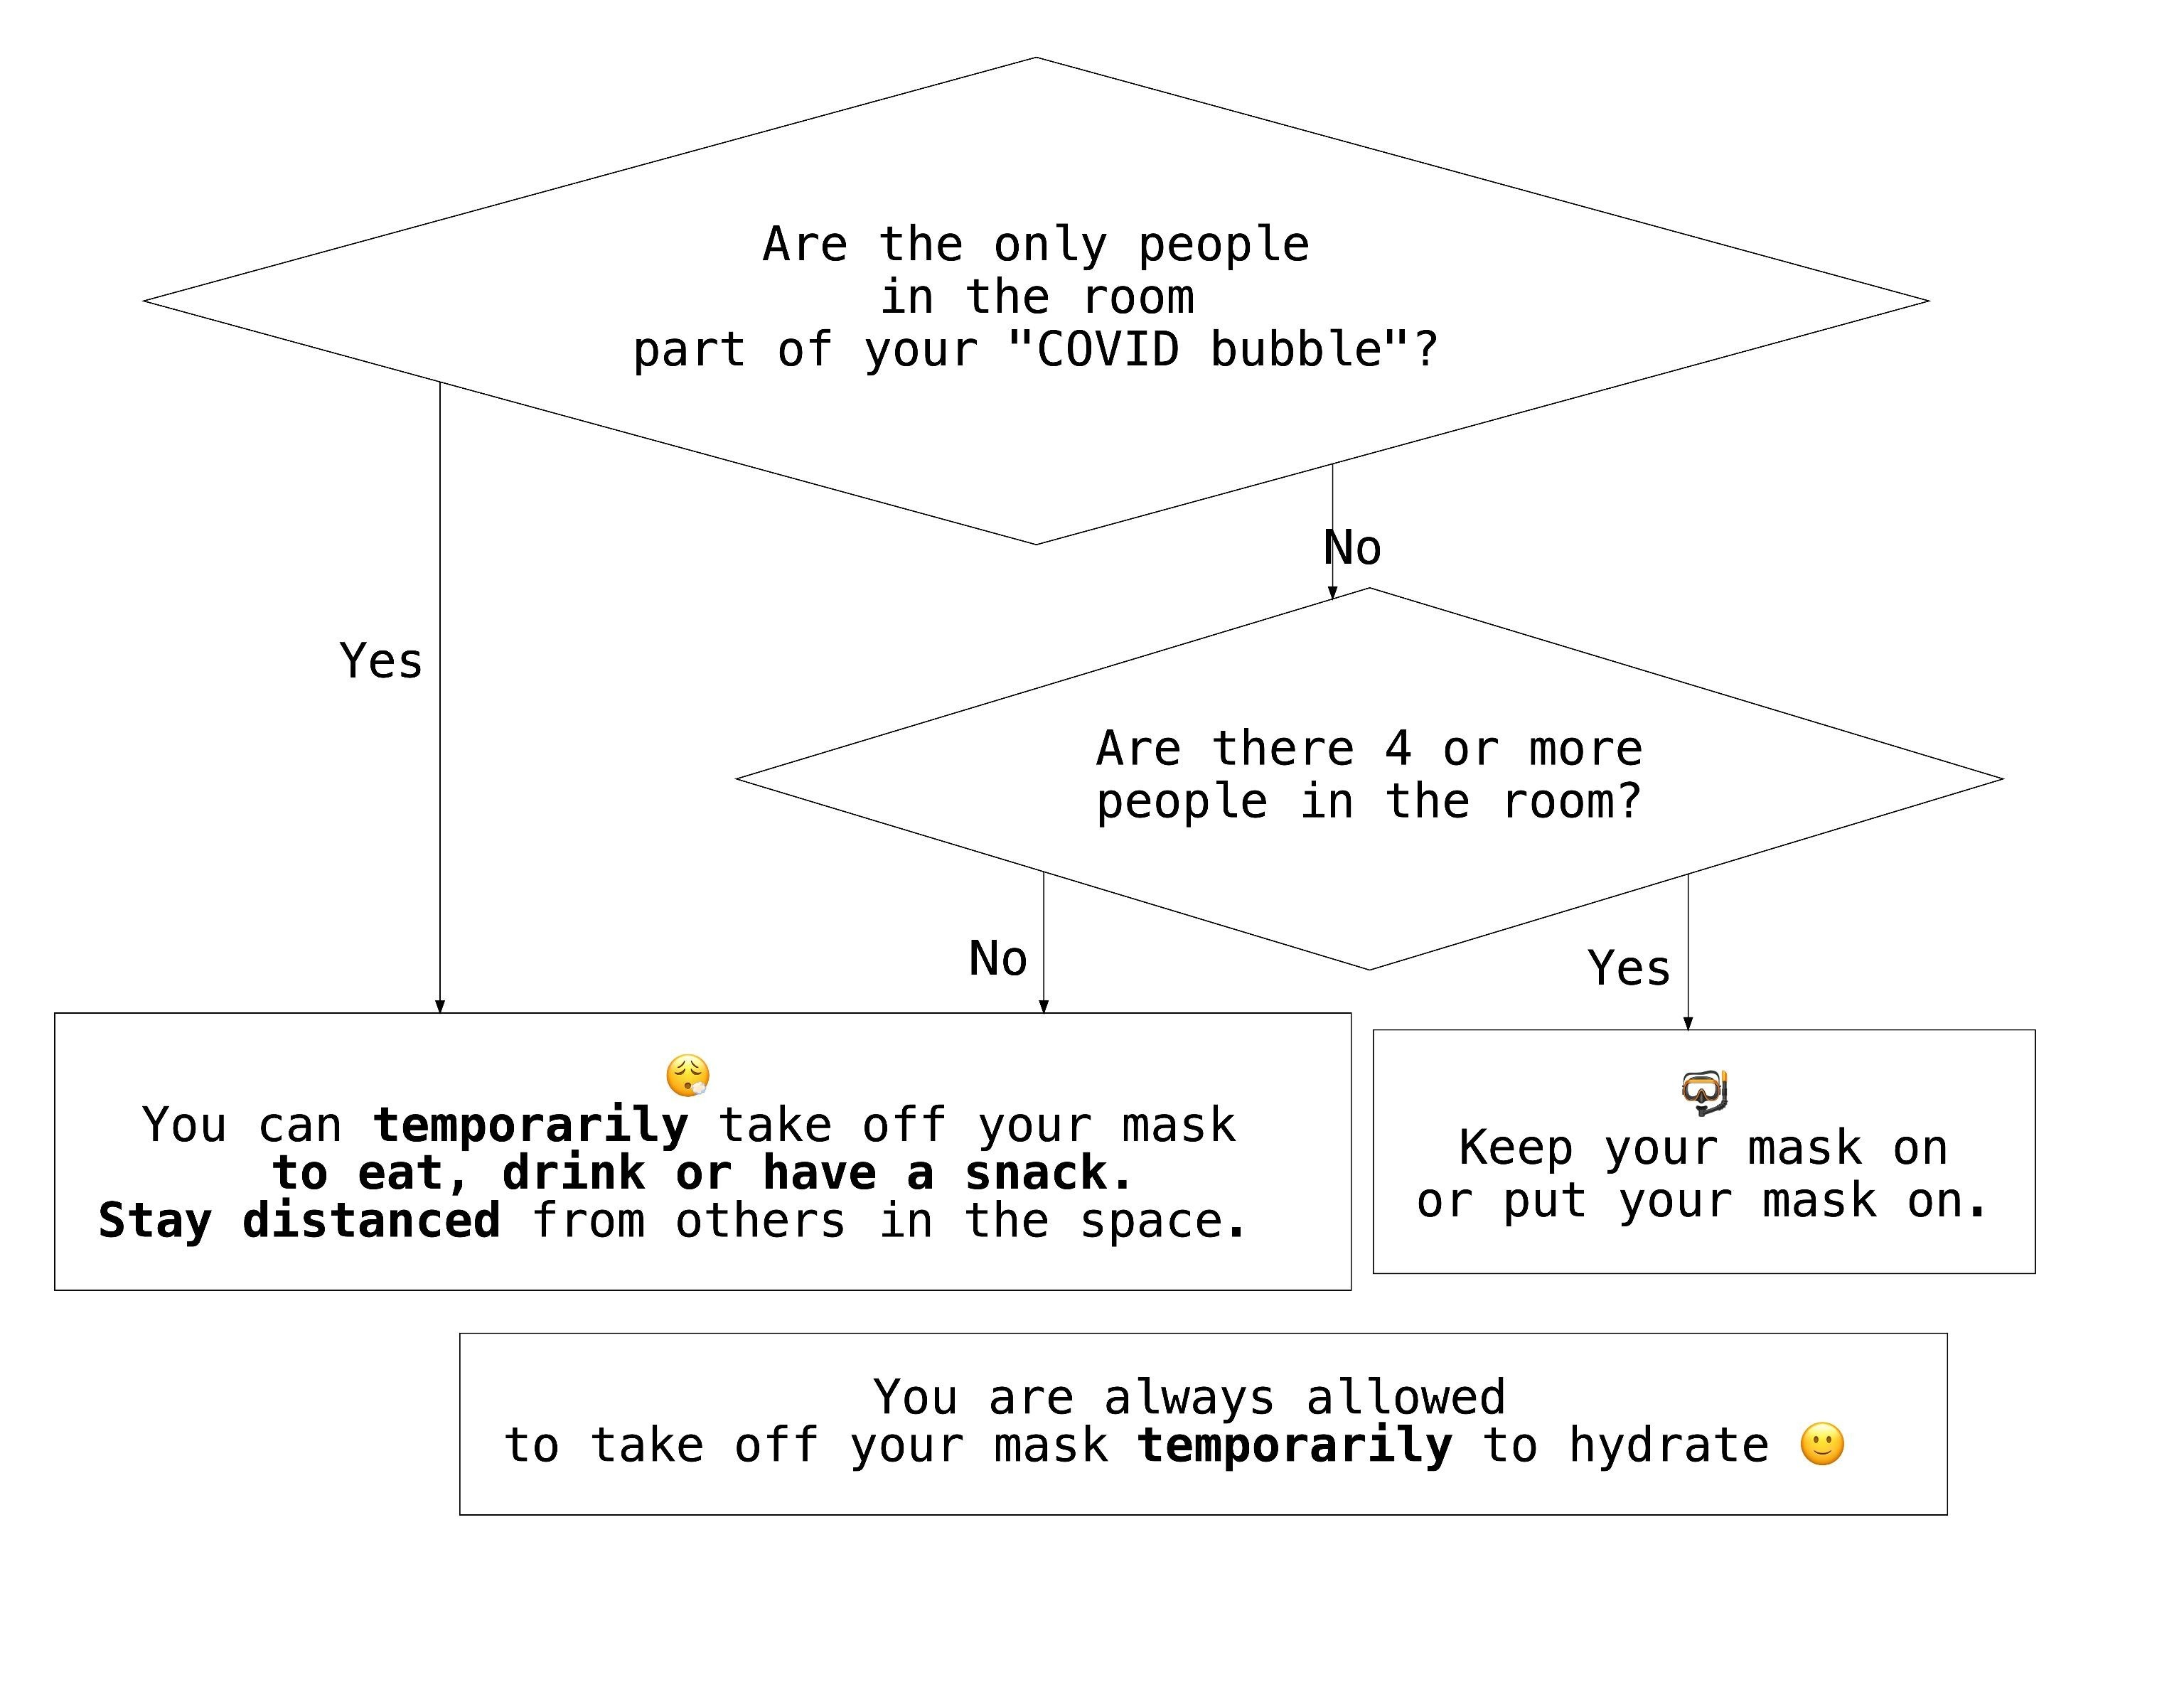
\includegraphics[scale=.175]{covidChart}
\end{center}

failure to do is considered a Moderate violation.

\section{Officers and Official Formalities}
\begin{itemize}
	\item If you observe any violation of ACM rules, contact an ACM officer. Contact information for these individuals can be found on the Officer List posted on the fridge and the door.
	\item If you would prefer to remain anonymous, you can use the ACM Suggestion Box at \url{https://z.umn.edu/suggest_acm}
\end{itemize}

\section{Violations and Consequences}
\subsection{Minor Violations}
\begin{itemize}
	\item Minor violations include a violation of one of our rules that does not seriously threaten the well-being of people, property, or propriety.
	\item Minor violations will result in a warning.
	\item If more than one rule violation occurs, a meeting with officers or University staff will be arranged.
\end{itemize}

\subsection{Moderate Violations}
\begin{itemize}
	\item Moderate violations include most violations of University policy, as well as actions that threaten the well-being of people, property, or propriety.
	\item Moderate violations will result in probation.
	\item Second time violations of this type may result in suspension of membership.
\end{itemize}

\subsection{Major Violations}
\begin{itemize}
	\item Major violations include violations of local, state or federal law, as well as violations of University policy that seriously threaten or actually injures the well-being of people or property.
	\item Major violations will result in a meeting with University staff and potential suspension or expulsion.
	\item A second major violation will result in immediate expulsion from the organization.
\end{itemize}

\end{document}
